\documentclass[a4paper]{article}
\usepackage{style}
\usepackage{mcode}
\usepackage{tabularx}
\usepackage{pdfpages}

\setlength{\droptitle}{15em}
\title{Projekt 2\\ EIT060}

\author{Alexander Najafi (elt12ana)\\Tobias Mähl (har11tma)\\Simon Rydebrink (dat14sry)\\ Sebastian Karabeleski (dat12sk1)}

\date{2016-03-03}

\begin{document}

\maketitle
\newpage

\tableofcontents
\newpage

\section{Introduktion}
Denna rapport presenterar en lösning för att hantera ett journaler på ett sjukhus av ett säkert system. Vi kommer även tydligt och genomgående beskriva vår implementering av detta system.

En simulerad databas kommer att användas för att förvara journalerna. De olika sorters roller vi tagit hänsyn till när vi utformade systemet är:

\begin{itemize}
\item
Patient: En patient kan ha en eller fler journaler i systemet och kommer alltid att ha rättigheten att läsa dem. 

\item
Läkare: En läkare får både läs- och skrivrättigheter till alla sina patienters journaler samt även läsrättigheter till alla patienters journaler inom sin avdelning. Endast en läkare har också möjligheten att skapa en ny journal till en patient.

\item
Sjuksköterska: En sjuksköterska kommer att ha läs- och skrivrättigheter till alla patienter registrerade till sig och även sjuksköterskan har läsrättigheter till patienters journaler inom sin avdelning.
\end{itemize}

\section{Arkitekturell överblick}
Implementationen av journalsystemet för denna uppgift implementerades med hjälp av en central server och en implementation av en klientmjukvara. Klientmjukvaran skulle kunna vara implementerad på många olika sätt och plattformar så som för t.ex. mobiltelefoner men för denna uppgift valdes det att implementera en klient för datorer som var helt terminalbaserad. För kommunikationen mellan servern och klienten utvecklades en specifikation för ett JSON protokoll. JSON, som är ett open-source program framtaget för att automatisera parsing av meddelanden, implementerades för att kunna sköta kommunikationen på ett enkelt och strukturerat sätt. Det valdes för att standarden redan används flitigt och det finns många implementationer av parsing för många olika plattformar, vilket i sin tur skulle kunna göra att klienter för fler plattformar utvecklades.

\subsection{Server}
\subsubsection{Överblick}
Servern är den centrala delen i journalsystemet. Det är servern som håller reda på alla patienter, doktorer, sköterskor, journaler, inloggningar osv. I servern finns en implementation av en databas som innehåller alla journaler, användare osv. I implementationen implementerades databasen helt i internminnet för denna uppgift. Varje gång servern startar upp stoppas det in testdata i dess databas. Ingen information som sparas i databasen finns kvar om den skulle startas om. I ett verkligt system skulle så klart detta kunna implementeras med hjälp av t.ex. en MySQL databas. 

För att kunna kommunicera med servern måste en klient autentisera sig. Detta sker genom en tvåstegsverifikation där det ena steget är en autentisering med SSL-certifikat och den andra är med ett användarspecifikt lösenord. Säkerhetsaspekterna och detaljerna kring detta beskrivs nedan.

\begin{figure}[H]
	\centering
	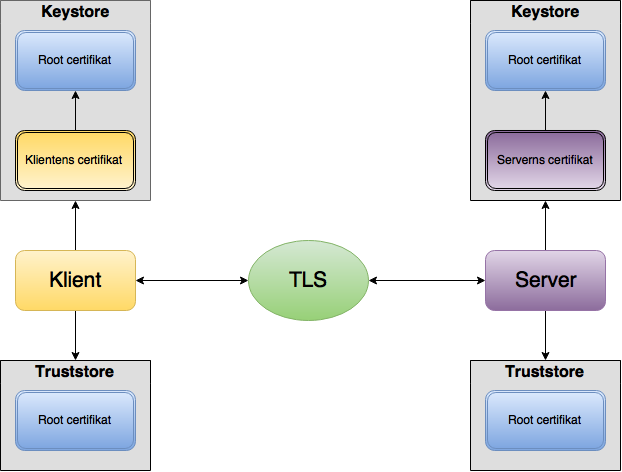
\includegraphics[width=0.7\textwidth]{sslcon.png}
	\caption{Diagram över hur systemet använder SSL.}	
	\label{bild}
\end{figure}

För att en klient ska kunna skicka förfrågningar till servern om att utföra uppgifter måste denna autentisera sig. Efter en lyckad autentisering genereras en token av servern som skickas tillbaka till klienten. Denna token måste skickas med varje förfrågan som klienten gör till servern. På så sätt kan servern veta precis vem som gör en förfrågan och baserat på detta bestämmer servern om personen får lov att utföra uppgiften (som t.ex. kan vara att skapa en ny patient, uppdatera patientuppgifter eller skapa en artikel i en patients journal) som specificeras.

I servern implementerades en statisk referensmonitor för att sköta kontrollen om en användare får utföra en viss uppgift. När en förfrågan kommer in till servern tar denna först reda på vilken typ av uppgift den ska utföra. Efter detta kontrollerar den om användaren som försöker utföra uppgiften har rätt att göra detta. Om kontrollen går igenom så utförs uppgiften och servern skickar tillbaka ett passande svar till klienten. 

Vid uppkoppling mellan servern och klienten går det till som enligt nedan. 
Klienten skickar en förfrågan till servern som svarar med sitt certifikat. 
Klienten verifierar certifikatet eftersom det är signerat av en tillförlitlig CA och skickar tillbaka sitt eget certifikat. 
Servern verifierar klientens certifikat och uppkopplingen räknas nu som säker och delandet av information kan börja. 
I detta utbyte av information har klient och server kommit överens om vilken krypteringsalgoritm som skall användas för att dela information. 

\subsubsection{Implementation}
I UML-diagrammet nedan syns de klasser som är essentiella för servern. Servern ser alla användare som personer, skillnaden mellan de olika personerna så som, doktorer, patienter och sköterskor är dess roll i systemet. De olika användarna har olika roller, och olika roller får göra olika uppgifter. Vilka uppgifter som vilka roller får utföra sköts av referensmonitorn. Till skillnad från patienter och statliga organisationer så har doktorer och sköterskor även en avdelning som tillhör deras användare. 

Programmet består av tre paket. UML-diagrammet visar visar common-paketet. Ett paket med klasser som både servern och klienten känner till. Common-paketet hanterar kommunikationen och mellan server och klient och där ligger även den intelligens som används av både server och klient. 
I server-paketet och klient-paketet ligger intelligens som är specifik för respektive funktion. Tillexempel hur klienten skall skicka användarens input till servern, och hur servern skall ta emot och behandla den info som klienten skickar.

\begin{figure}[H]
	\centering
	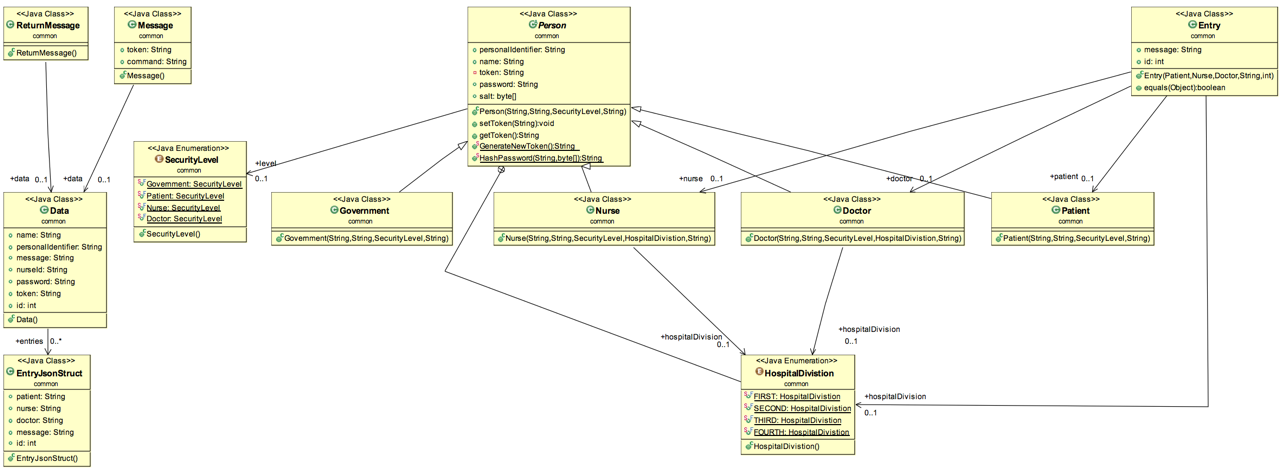
\includegraphics[width=1.0\textwidth]{uml.png}
	\caption{UML diagram över servermjukvaran.}	
	\label{bild}
\end{figure}

\subsection{Textbaserad klient}
Klienten som implementerats för denna uppgift är en enkel, helt textbaserad klient med syfte att demonstrera servens implementation. När klienten startas ansluter denna till servern och autentiserar sig själv med hjälp av ett x509 certifikat. När en användare sedan använder klienten för att logga in skriver denna in sitt personnummer och lösenord som skickas till servern. Vid en lyckad autentisering gäller det för klienten att hålla koll på den token som servern då skickar tillbaka.

Klienten tar inmatning från användaren i form av ett komando och ber sedan om ytterligare information som behövs för det valda komandot. När användaren matat in all information som behövs, så skapar klienten ett JSON meddelande som skickas till servern. När klienten får ett svar från servern tolkar den detta och ger ett användarvänligt meddelande till användaren. När användaren bestämmer sig för att logga ut skickar klienten ett meddelande till servern om att användaren ska loggas ut. Efter detta är den token som klienten använt under sessionen värdelös och kan inte användas mer. För att göra fler förfrågningar till servern måste en ny token genereras av servern genom att en användare loggar in igen.

\section{Etisk diskussion}
För att en vettig diskussion i etik och moral angående journalsystemet ska kunna genomföras måste det först etableras var denna fråga skapas.

Patienter tar sig till en läkare eftersom de har ett problem som de hoppas läkaren kan hjälpa till att korrigera. Läkaren ska då genomföra vården av patienter med avsikt och skyldighet att göra alla rimliga ansträngningar för att hjälpa dem. Men varje medicinskt fall är inbäddad i ett större sammanhang för de personer och institutioner som är inblandade. Detta större sammanhang påverkas av de beslut som fattas av eller om patienten. Dessa beslut har psykologiska, känslomässiga, ekonomiska, juridiska, vetenskapliga och religiösa påverkan på andra som kan vara av avgörande betydelse för patienten. Därför sparas medicinska journaler med omfattande säkerhet, för om någon utomstående skulle få kännedom om dessa beslut, kan det få betydande konsekvenser de inblandade.

Under designstadiet med kunden bör det informeras var säkerhetsstandarden enligt Personuppgiftslagen ligger och vilken miniminivå säkerheten på systemet bör hålla. Då kan det också rekommenderas och diskuteras med kunden vad som kan vara lämpligt utöver denna. Detta beroende på vilka risker som finns redan nu och vilka som kan bli aktuella i framtiden. Men i slutändan så är det alltid kunden som måste ta ett beslut då det är dem som ska använda och betala för det. Ditt ansvar som ingenjör är att informera och rekommendera så att det bästa beslutet för kunden kan tas.

För att uppnå en design för att ge användare olika behörigheter i ett journalsystem, så hade vi valt att ge alla användare väldigt fördefinierade roller. För att tillämpa “principle of least privilege” på ett smidigt och enkelt sätt. Försöka undvika specialfall och hålla administrationen av systemet så enkel som möjlig.

De olika aktörerna vid upphandling och användning av ett sjukhusjournalsystem har alla lite olika etiska dilemma de står inför. När systemet ska köpas upp måste sjukhusledningen se till att det uppfyller alla lämpliga lagar för att hantera den aktuella information, det vill säga Personuppgiftslagen etc. Utöver det så måste de väga ekonomiska fördelar mot olika säkerhetsaspekter för systemet. För ingenjören/designern/implementeraren så kan det vara smidigt att inte lämna över all access till systemet när det anses färdigt. Utan att ha kvar en bakdörr eller liknande för att kunna rätta till saker i efterhand. Även om det skulle vara smidigt så är det tillgänglighet mot integritet. Medans för sjukhuspersonalen så gäller det att inte utnyttja dem designvalen som har gjorts för systemet.  Detta även om dem skulle ha tillgång till någon typ av information enligt systemet så betyder inte det alltid att det är etiskt rätt att använda den. Sen om dem skulle finna buggar eller liknande som kringgår säkerhetsaspekterna under användning, så kan det tyckas att dessa ska rapporteras och inte utnyttjas.

\subsection{Rättigheter}
I ett fiktivit, optimalt system skulle en rättighetstabell kunna se ut som den nedan.

\begin{tabularx}{\textwidth}{|l|X| X | X | X |}
\hline
\textbf{Person} & \textbf{Läsa} & \textbf{Skriva} & \textbf{Ändra} & \textbf{Radera} \\
\hline

\textbf{Patient} & Ska kunna läsa all info om sig själv & Ej & Ej & Ej \\
\hline

\textbf{Sköterska} & \multicolumn{2}{p{5.0cm}|}{Ska kunna läsa och skriva journaler på patienter som är inskrivna på sjukhuset eller de som de någon gång behandlat} & Ska kunna ändra det som han skapat & Ej \\
\hline

\textbf{Läkare} & \multicolumn{2}{p{5.0cm}|}{Ska kunna läsa och skriva journaler på patienter som är inskrivna på sjukhuset eller de som de någon gång behandlat} & Ska kunna ändra det som han skapat & Ej \\
\hline

\textbf{Myndighet} & Ej & Ej & Ej & Ja, vad som helst \\
\hline

\end{tabularx}

\section{Säkerhetsutvärdering}

För att hålla systemet säkert har vi tagit flertalet åtgärder. Den första är att uppkopplingen mellan klienten och servern kräver en SSL uppkoppling. Detta uppnås genom att server och klient båda litar på samma certifikat. Detta är vår ena faktor i vår tvåfaktorsautentisering. SSL uppkopplingen låter oss skicka information mellan klient och server på ett säkert sätt och vi kan vara säker på att informationen når fram till rätt server samt att informationen kommer fram oläst och oförändrad. Certifikaten är unika för varje användare, användaren får ha sitt certifikat lagrat på t.ex. ett USB-minne eller i sin dator för att lösningen ska kunna fungera. 

Uppkopplingen använder SHA1 med RSA som signaturalgoritm. Detta är inte den absolut säkraste uppkopplingen, men den uppfyller enligt oss rimliga säkerhetskrav. SHA1 är i teorin knäckt då det skulle vara möjligt att hitta en kollision i hashningen men detta är ännu inte genomfört rent praktiskt.

När en säker uppkoppling är upprättad når vi steg två i vår tvåfaktorsautentisering. Användaren ombeds nu att ange sitt användarnamn och lösenord. 
När användaren är inloggad vet systemet vilka rättigheter användaren har och ger då användaren rättigheter kopplade till dennes behörighet till de funktioner som den bör ha.

Lösenordet får användaren välja själv. Men uppmanas att välja ett lösenord som innehåller både gemener, versaler, samt siffror eller specialtecken. 
Detta innebär en svaghet och en säkerhetsrisk i vårt program, då ett dåligt valt lösenord skulle möjliggöra en hackare att utföra en brute force attack, dictionary attack eller en rainbow table attack på en rimlig tid.

När en säker uppkoppling har etablerats och en användare har autentiserat sig själv tilldelas denne en token (en lång slumpmässigt vald sträng), en token som användaren kommer att skicka med i alla förfrågningar som den gör. När servern mottager en förfrågan, till exempel att skriva ett nytt journalinlägg så kontrollerar serven den token som användaren har skickat med.

\subsubsection{Styrkor och svagheter}
Systemet för journaler har utvecklats på sådant vis så att följande attacker \emph{inte} kan utföras på systemet. 

\begin{description}
\item[Man-in-the-middle attack] Att försvara sig mot Man-in-the-middle attacker är väldigt svårt utan en separat, säker, kanal för verifiering. Genom att använda SSL-anslutningar och certifikat, som är signerade av gemensam certifikatutfärdare(CA), så går denna attacken också att undvika. En “eavesdropper” hade behövt lura CA:n att signera sitt certifikat med serverns namn. Detta borde inte vara möjligt då CA:n borde kolla alla certifikat den signerar.
\item[Eavsdropping] Denna attacken undviks helt enkelt genom att använda SSL-protokollet.
\item[Fake Certifkat] Eftersom vi använder en enda certifkatsutfärdare(CA) som signerar alla certifikat, så blir inga certifikat signerade av någon annan.

\item[Brute-Force attack] Såvitt man hållit sig till våra förslag om hur ditt lösenord ska vara utformat så borde inte brute-force attacker vara en fara. Med de specifikationer vi utformade tar det mer än ett år innan man kan knäcka lösenordet med en brute-force attack och då måste ändå certifikatet förnyas.

\end{description}

\begin{description}

\item[Spoofed Client] Om en anfallare skriver en låtsasklient och lurar en användare, låt oss kalla henne Alice, att använda den så har vi inget skydd mot det. Det allvarligaste en anfallare kan göra i detta fallet är att stjäla all patientinformation som Alice har åtkomst till. Oturligt nog det enda är att försäkra sig att man har laddat ner rätt klient är att besöka sjukhuset hemsida genom en SSL-anslutning eller på något annat säkert vis.

\item[Dictionary attack] Om man håller sig undan att använda vanliga ord blir en dictionary attack meningslös. Det är däremot upp till användaren att välja sitt lösenord och vi kräver inte hur de utformar sitt lösenord. Man skulle kunna lägga till att man bara får t.ex. skriva in sitt lösenord var femte sekund, och då tar den attacken längre tid.

 \end{description}
 
 \subsection{Journalernas tillgänglighet}
 
Inledningsvis, så förser vi konfidentialitet till våra patienter. Konfidentialitet innebär skyddet av personlig data och detta förses bara genom att låta auktoriserade användare läsa de olika journalerna.
Dessutom, när man skapar en journal, så är det enda som kan ändras av en auktoriserad användare är patientens information, inte av den som behandlar den, vilket tillför integritet. Detta förhindrar folk från att ändra vem som behandlar patienten till sin egen fördel. T.ex. för att en icke auktoriserad användare tillåts komma åt det.

\newpage

\section{Appendix}
\subsection{Peer-reviews}
Nedan finns de peer reviews som inkommit från de andra grupperna. 

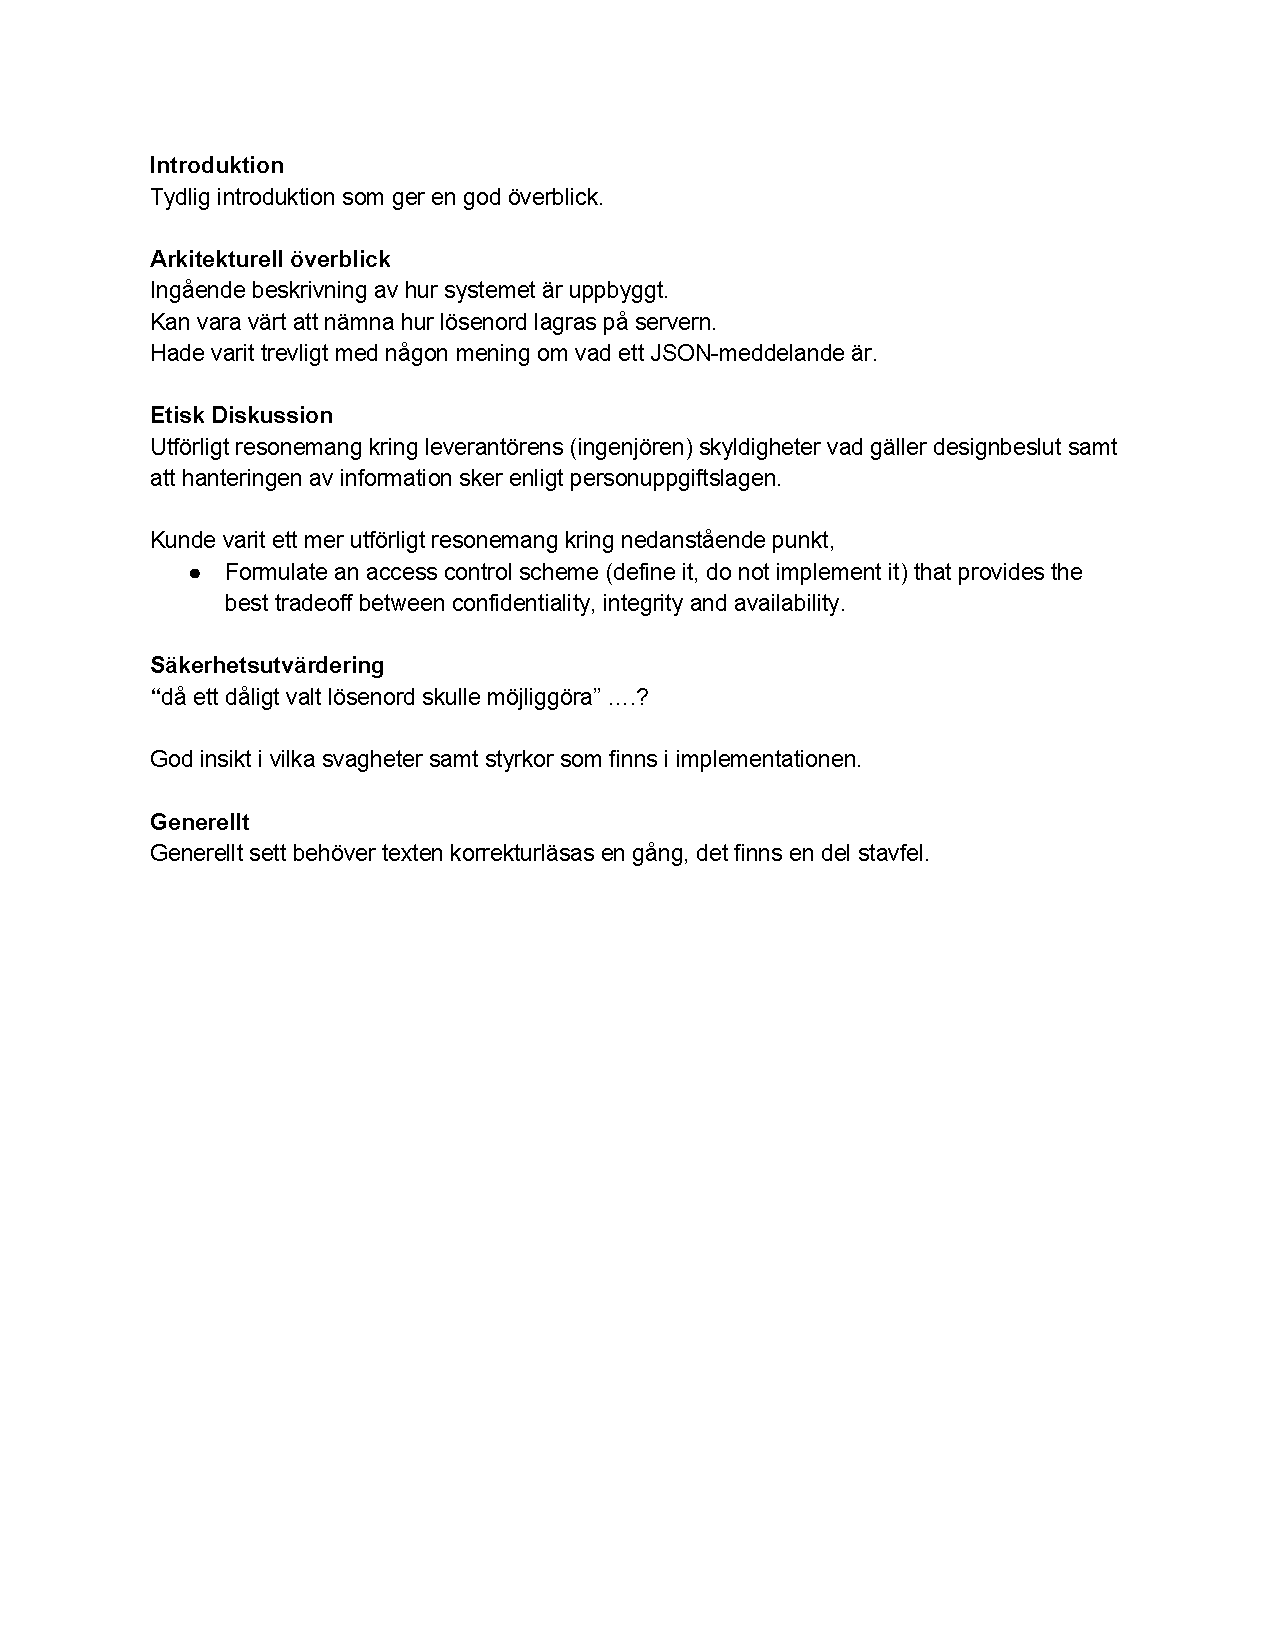
\includepdf[pages={1}]{review1.pdf}

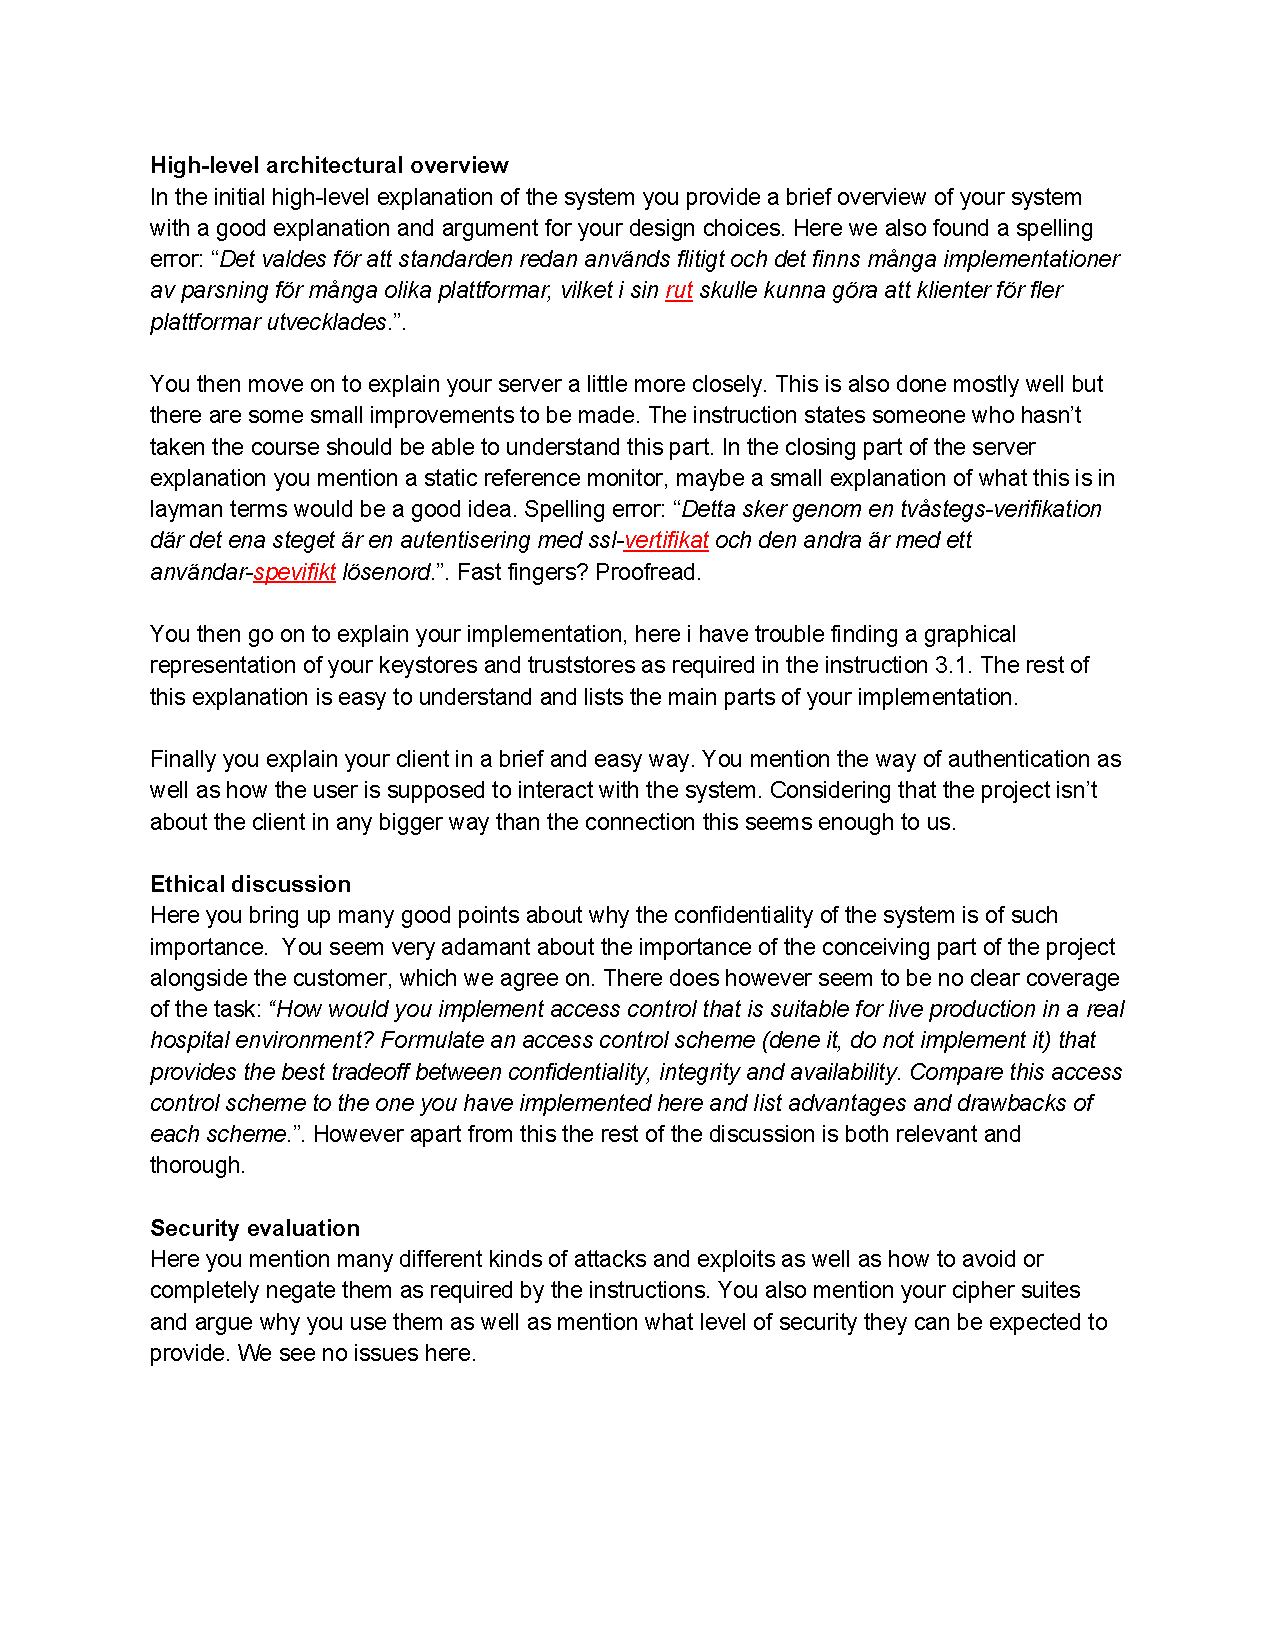
\includepdf[pages={1}]{review2.pdf}

\newpage
\subsection{Gjorda förbättringar}

Efter att ha mottagit rapporter om förbättringar från två andra grupper så har vi främst förbättrat språkliga misstag så som stavfel och meningsbyggnader. Vi har förbättrat vår rapport på så sätt att vi har diskuterat och skapat en tabell över ett optimalt kontrolschema för ett system på ett verkligt sjukhus.

Efter att ha haft en code review med en annan grupp så gjorde vi inga ändringar förutom ett utskriftsmeddelande som var fel i klienten. Vi ordnade även så att lösenord som skrivs in i terminalen maskeras och inte syns. 

Vi har uppdaterad UML diagramet i rapporten efter den senaste versionen av koden.

\subsection{Code review och Project contributions}
Nedan finns dokument för code review och project contribution.

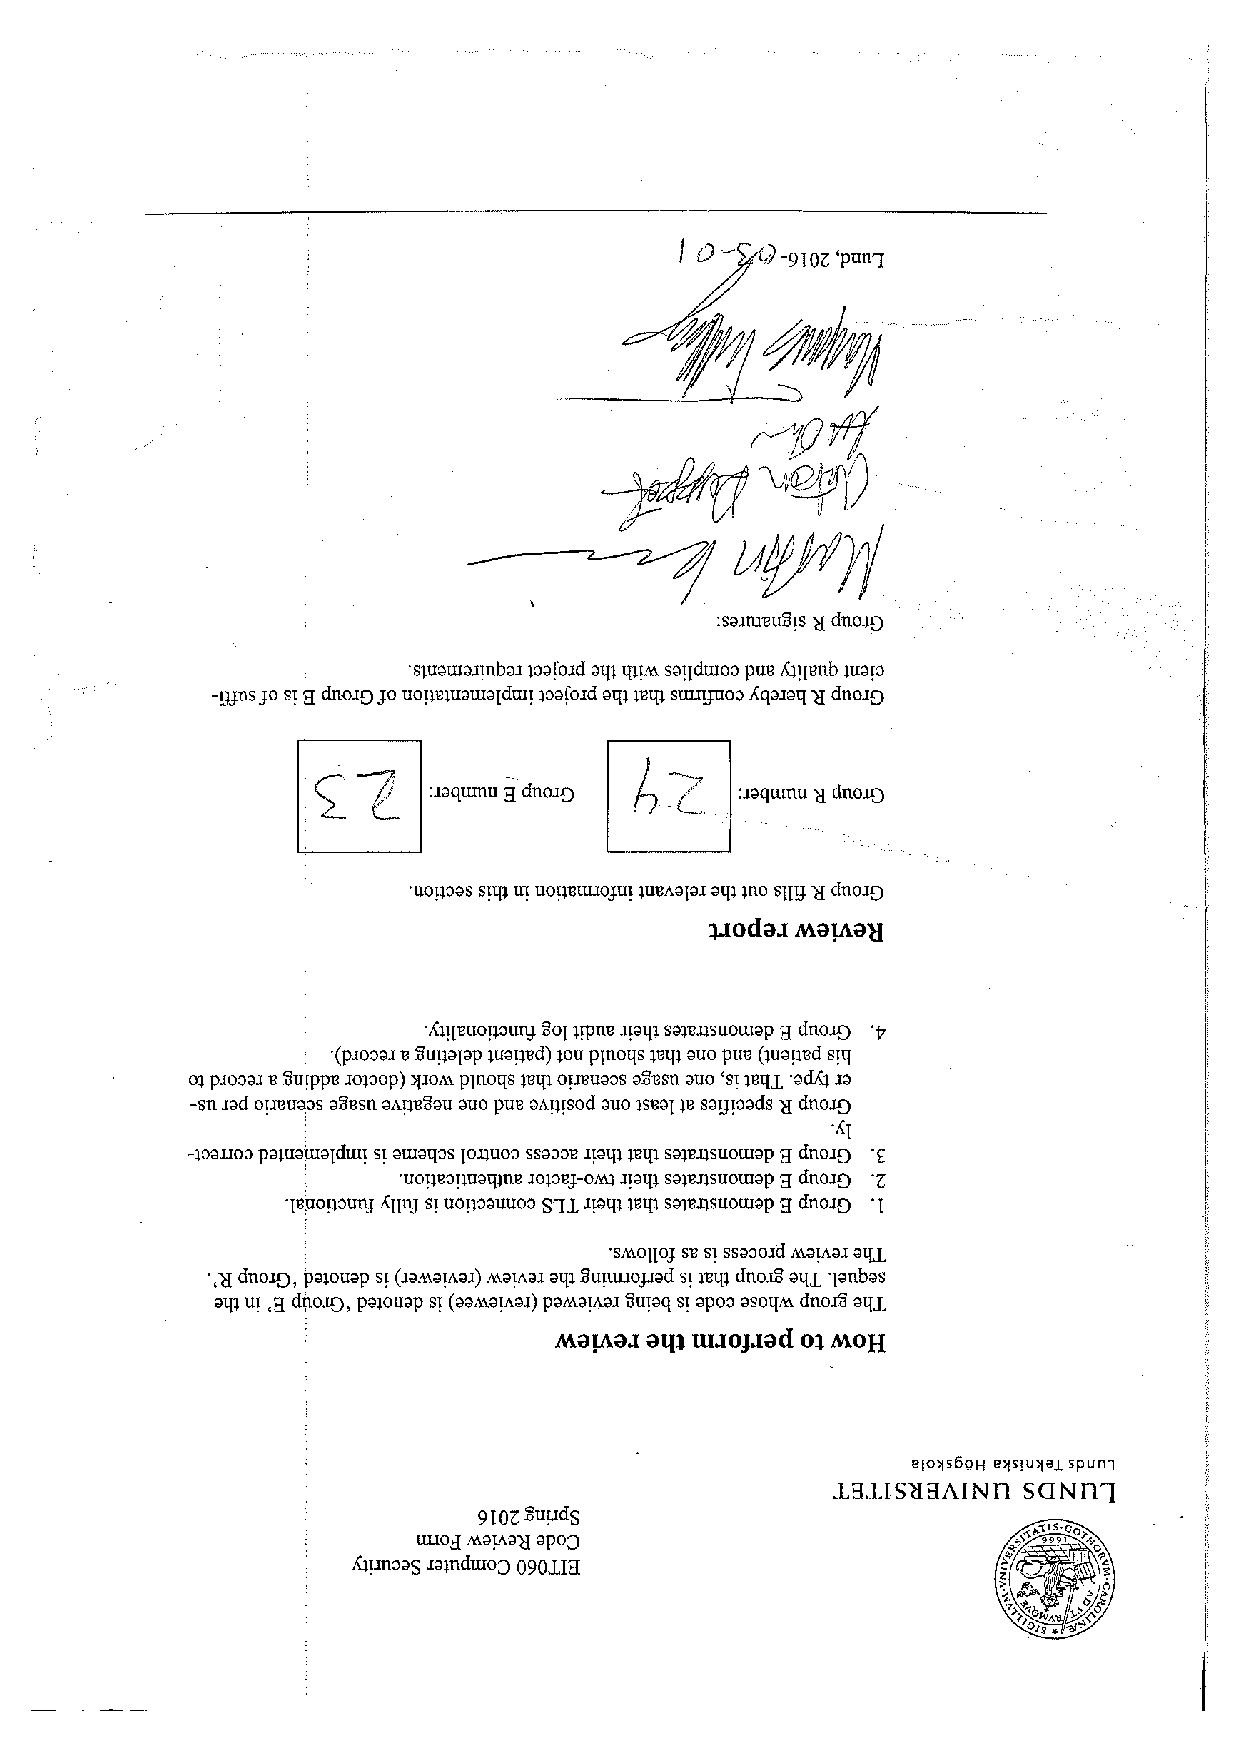
\includepdf[pages={1},angle=180]{code_review}

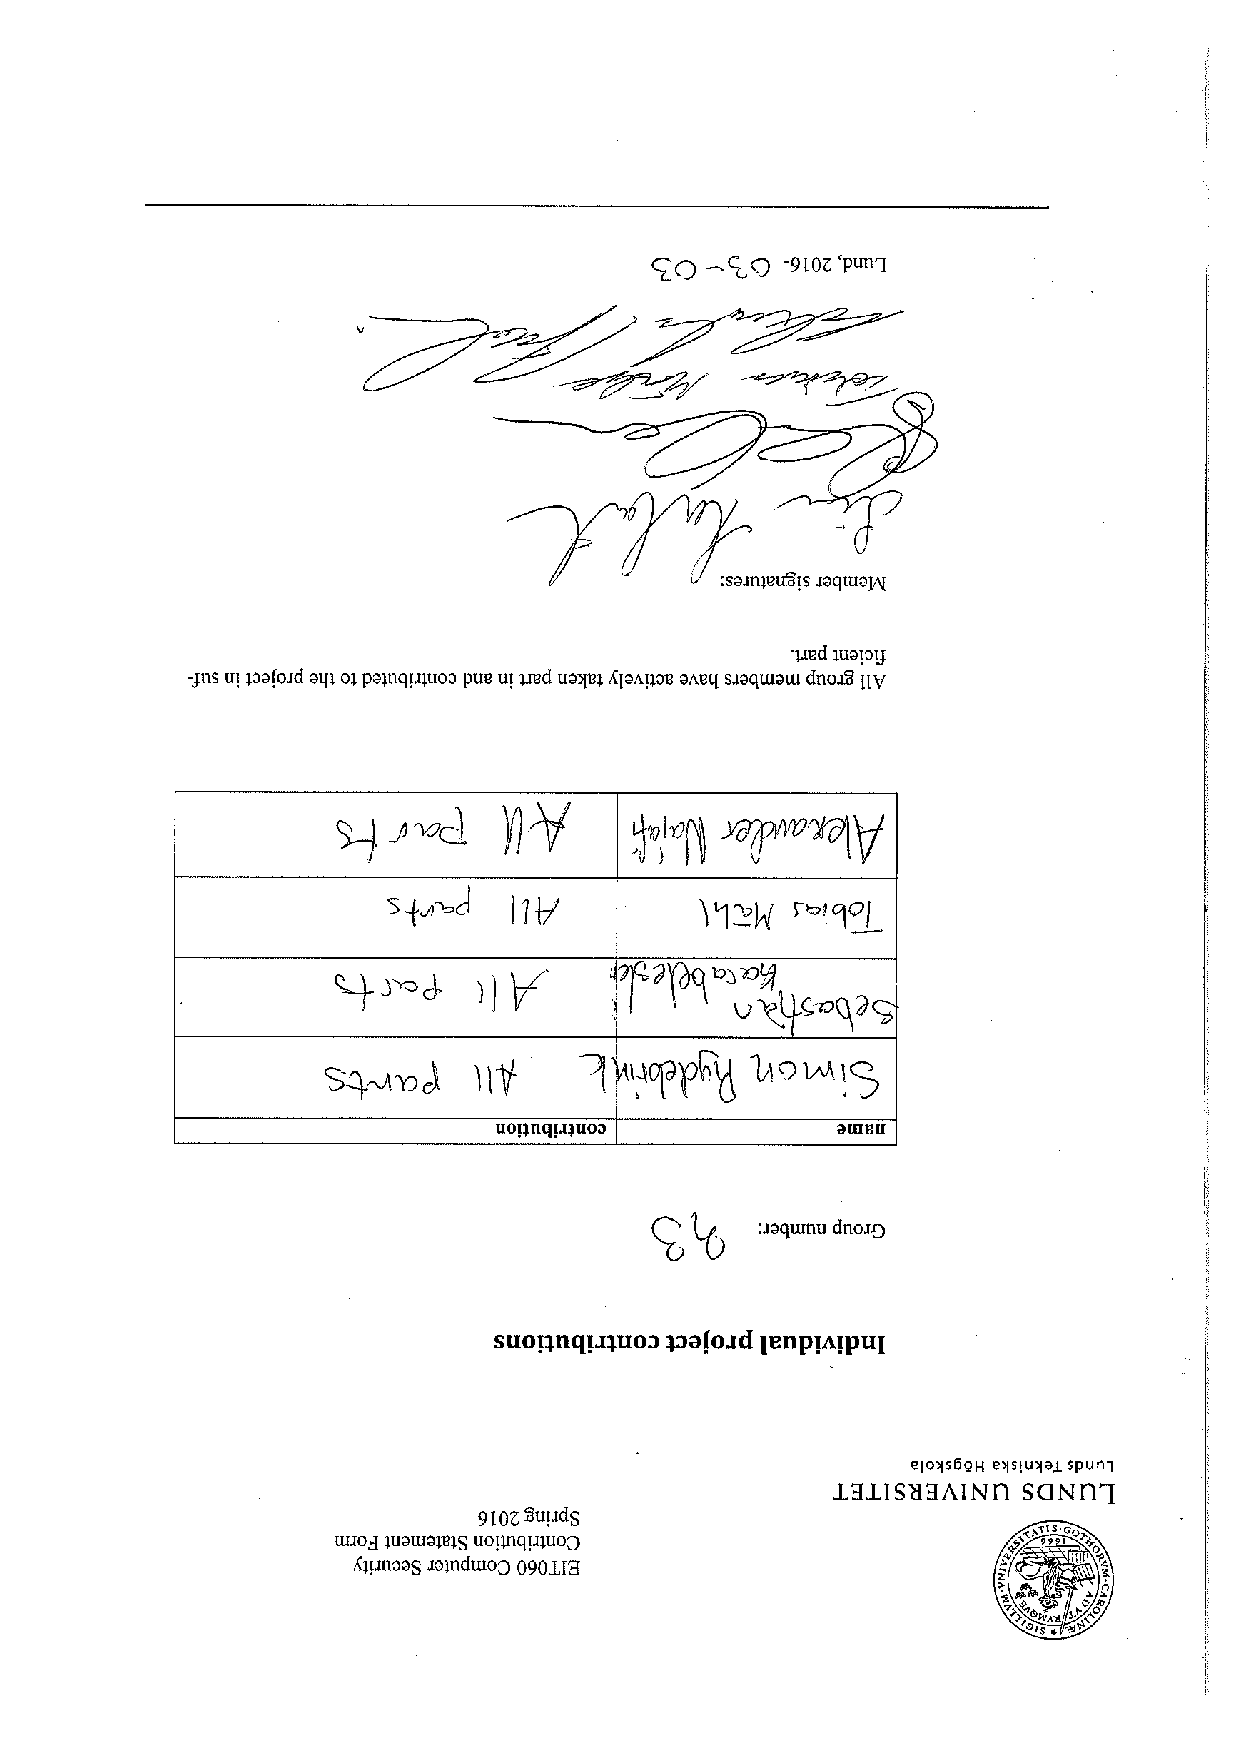
\includepdf[pages={1},angle=180]{proj_contrib}

\end{document}  